\documentclass{standalone}
\usepackage{tikz}

\begin{document}

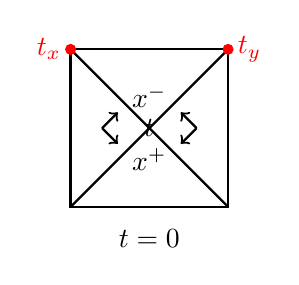
\begin{tikzpicture}[scale=2]
    % Draw the square
    \draw[thick] (0,0) -- (1,0) -- (1,1) -- (0,1) -- cycle;
    
    % Draw the diagonal lines
    \draw[thick] (0,0) -- (1,1);
    \draw[thick] (0,1) -- (1,0);
    
    % Mark the points on the top corners
    \fill[red] (0,1) circle (1pt) node[left] {$t_x$};
    \fill[red] (1,1) circle (1pt) node[right] {$t_y$};
    
    % Label the regions
    \node at (0.5, 0.7) {$x^-$};
    \node at (0.5, 0.3) {$x^+$};
    
    % Label the time variable
    \node at (0.5, 0.5) {$t$};
    \node at (0.5, -0.2) {$t = 0$};
    
    % Arrows for the time variable
    \draw[->, thick] (0.2, 0.5) -- (0.3, 0.6);
    \draw[->, thick] (0.8, 0.5) -- (0.7, 0.6);
    \draw[->, thick] (0.2, 0.5) -- (0.3, 0.4);
    \draw[->, thick] (0.8, 0.5) -- (0.7, 0.4);
    
\end{tikzpicture}

\end{document}